\documentclass[11pt,a4paper]{article}

\usepackage[a4paper,margin=1in]{geometry}
\usepackage[utf8]{inputenc}
\usepackage[T1]{fontenc}
\usepackage{lmodern}
\usepackage{graphicx}
\usepackage{booktabs}
\usepackage{longtable}
\usepackage{array}
\usepackage{xcolor}
\usepackage{hyperref}
\usepackage{caption}
\usepackage{enumitem}
\usepackage{fvextra}
\usepackage{float}
\usepackage{tikz}
\usetikzlibrary{arrows.meta,positioning}

\hypersetup{
  colorlinks=true,
  linkcolor=blue!50!black,
  urlcolor=blue!50!black,
  citecolor=blue!50!black
}

\setlist[itemize]{leftmargin=1.4em}
\setlist[enumerate]{leftmargin=1.6em}
\renewcommand{\arraystretch}{1.18}
\DefineVerbatimEnvironment{Prompt}{Verbatim}{
  breaklines=true,
  breakanywhere=true,
  fontsize=\footnotesize,
  frame=single,
  framesep=3mm,
  rulecolor=\color{black!30}
}

\title{\textbf{Virtual Academic Advisor}\\
\large Agentic LLM System for GSU Computer Engineering Graduation Analysis}
\author{INF473 Project Report}
\date{May 9, 2026}

\begin{document}
\maketitle

\begin{abstract}
This report documents the completed Virtual Academic Advisor project, an agentic
LLM-based system that evaluates unstructured Galatasaray University Computer
Engineering transcripts against graduation requirements. The implemented system
combines a language-model transcript parser, a rule-based academic knowledge
base, independent verification agents, and a tool-augmented master
reporting agent. The result is a web application that accepts transcript text,
normalizes academic records, checks mandatory courses, ECTS, GPA, language, and
elective requirements, and produces an advisor-style graduation report with
clear missing conditions.
\end{abstract}

\tableofcontents
\newpage

\section{Project Overview}

The project addresses a practical academic advising problem: students submit
transcripts as unstructured text, while graduation eligibility depends on a
structured interpretation of the official Computer Engineering curriculum. The
system therefore has three core responsibilities:

\begin{enumerate}
  \item extract reliable structured data from raw transcript text;
  \item compare that data with the GSU Computer Engineering graduation rules;
  \item generate a concise, human-readable report explaining whether the student
  satisfies the requirements and, if not, which conditions are blocking
  graduation.
\end{enumerate}

The official GSU ECTS page for the Computer Engineering undergraduate program
is the curriculum reference used by the project. The page lists the semester
curriculum, general graduation rules such as the minimum GPA requirement,
foreign-language requirement, and the rule that students below 240 ECTS must
complete missing credits with INF electives.\footnote{\url{https://ects.gsu.edu.tr/tr/program/programmedetails/12}}

\section{Project Motivation}

We chose this project because graduation eligibility is a practical and
high-impact problem for students. A student may have completed many courses but
still be blocked by a missing mandatory course, an elective-group rule, a low
GPA, insufficient ECTS, or a foreign-language requirement. Manually checking
these conditions is time-consuming and error-prone, especially when transcripts
include old course codes, repeated courses, failed courses, or curriculum
transition rules.

The project is also a suitable use case for an agentic LLM system. The input is
unstructured academic text, which is difficult to process with only static
forms, while the final graduation decision must remain deterministic and
explainable. Therefore, the project allowed us to combine the language
understanding capability of LLMs with rule-based verification. This combination
matches the academic advising domain: flexible parsing is useful, but the
decision itself must be based on explicit university requirements.

\section{System Scope}

The implementation is a full-stack application:

\begin{itemize}
  \item \textbf{Backend:} FastAPI service in \texttt{backend/main.py}.
  \item \textbf{Agent pipeline:} LLM-backed and rule-aware agent logic in
  \texttt{backend/agent.py}.
  \item \textbf{Knowledge base:} encoded GSU requirements in
  \texttt{backend/gsu\_requirements.py}.
  \item \textbf{Persistence:} SQLite database via SQLAlchemy models in
  \texttt{backend/models.py}.
  \item \textbf{Frontend:} React/Vite application under \texttt{frontend/src}.
  \item \textbf{Validation assets:} 20 transcript scenarios under
  \texttt{analysis-input-scenarios/}.
\end{itemize}

The system is an agentic academic-advising architecture. Its agents are not all
implemented in the same way: some are LLM-backed agents for language-intensive
tasks, and some are rule-verifier agents that execute the curriculum knowledge
base through Python. The scope of the application covers the complete advising
workflow from raw transcript submission to persistent analysis history. A
student can submit a plain-text transcript through the frontend, the backend
stores and deduplicates the input, the agent pipeline evaluates graduation
eligibility, and the result is returned as both structured data and an
advisor-style natural-language report. The system also exposes agent-level
verdicts, missing conditions, and course-level evidence so that the final
decision can be inspected rather than treated as an LLM answer.


\section{Agentic Architecture Design}

\subsection{High-Level Design}

The project follows a staged agentic workflow:

\begin{enumerate}
  \item \textbf{Input acquisition.} The frontend accepts pasted transcript text
  or a \texttt{.txt} file.
  \item \textbf{Input validation.} Client and server validation reject empty
  submissions and likely multi-transcript inputs.
  \item \textbf{Persistence and deduplication.} The backend stores the raw
  transcript and uses a SHA-256 text hash to avoid duplicate transcript rows.
  \item \textbf{LLM parsing.} \texttt{TranscriptParserAgent} transforms the raw
  transcript into typed JSON.
  \item \textbf{Independent verification.} Three rule-verifier agents evaluate
  course completion, ECTS, and broader graduation requirements.
  \item \textbf{Cross-examination.} Agents add short comments on how their
  findings relate to other agents' findings.
  \item \textbf{Master decision.} \texttt{MasterAgent} aggregates verdicts; the
  student is eligible only when all verifier agents pass.
  \item \textbf{Tool-augmented reporting.} The master report step may call a
  SQLite history tool to compare the current analysis with prior records.
  \item \textbf{Report review.} \texttt{ReportCriticAgent} polishes the final
  text and removes machine-like wording.
  \item \textbf{Presentation.} The frontend displays metrics, missing
  conditions, agent verdicts, course lists, history, and PDF export.
\end{enumerate}

\begin{figure}[H]
  \centering
  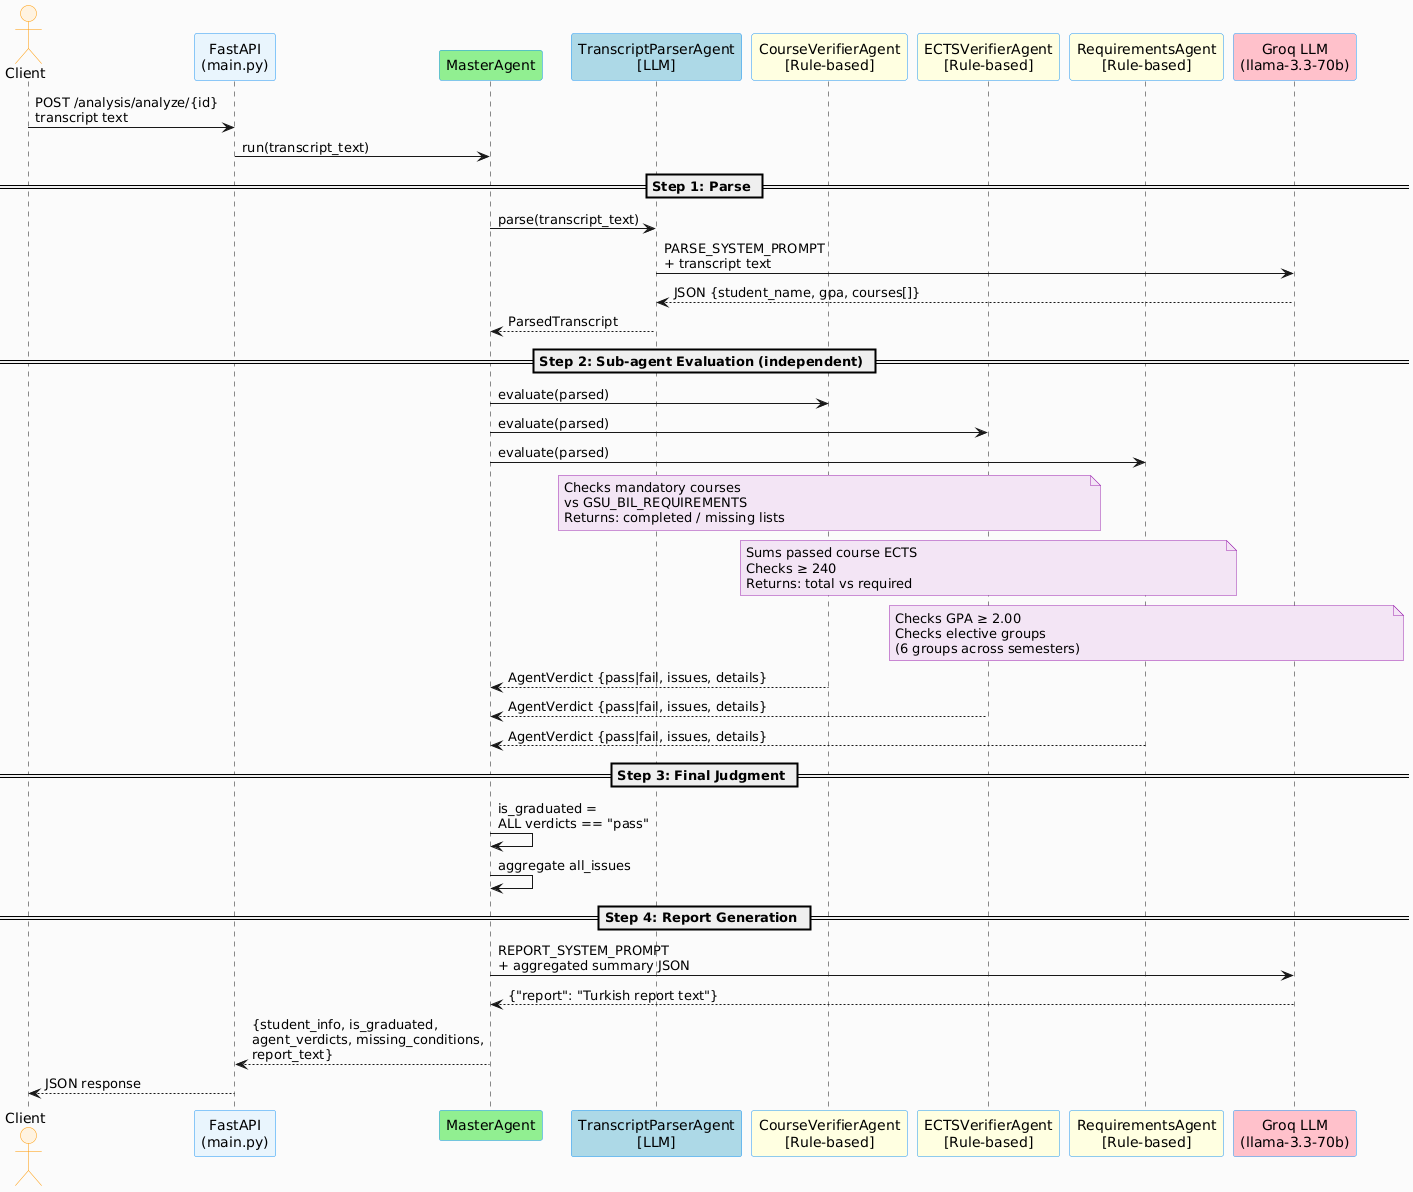
\includegraphics[width=0.95\textwidth]{sequence-diagram.png}
  \caption{Implemented sequence diagram from the project repository.}
  \label{fig:sequence}
\end{figure}

\section{Component Analysis}

\subsection{Backend API}

The FastAPI backend exposes the following main endpoints:

\begin{table}[H]
\centering
\begin{tabular}{lll}
\toprule
\textbf{Method} & \textbf{Endpoint} & \textbf{Purpose} \\
\midrule
\texttt{POST} & \texttt{/transcripts/upload} & Validate, hash, and store transcript text. \\
\texttt{POST} & \texttt{/analysis/analyze/\{id\}} & Run the agent pipeline for a transcript. \\
\texttt{GET} & \texttt{/analysis/\{id\}} & Retrieve a stored analysis result. \\
\texttt{GET} & \texttt{/analysis/history} & List recent analyses. \\
\texttt{DELETE} & \texttt{/analysis/\{id\}} & Delete an analysis and its transcript. \\
\bottomrule
\end{tabular}
\caption{Backend API surface.}
\end{table}

The backend also performs lightweight SQLite migration at startup, adding
columns such as \texttt{text\_hash} and \texttt{agent\_verdicts} for older
database files.

\subsection{Transcript Validation}

\texttt{backend/transcript\_validation.py} protects the pipeline from common
bad inputs. It detects multiple transcripts by checking repeated example
headers, conflicting student names, conflicting student numbers, and cumulative
ECTS resets in \texttt{Genel} rows. The same idea is mirrored in the frontend
upload page so the user receives fast feedback before the backend request.

\subsection{LLM Client Layer}

The LLM integration uses the Groq API. The model cascade is:

\begin{itemize}
  \item \texttt{llama-3.3-70b-versatile};
  \item \texttt{llama-3.1-8b-instant};
  \item \texttt{gemma2-9b-it}.
\end{itemize}

The shared \texttt{\_chat} wrapper uses temperature \texttt{0.0}. When no tools
are supplied, it requests JSON-mode output. When tools are supplied, it enables
native tool calling and lets the model decide whether to call the tool.

\subsection{Knowledge Base}

The knowledge base is implemented in \texttt{backend/gsu\_requirements.py} as a
Python dictionary named \texttt{GSU\_BIL\_REQUIREMENTS}. It contains:

\begin{itemize}
  \item minimum GPA: \texttt{2.0};
  \item minimum ECTS: \texttt{240};
  \item language condition: 12 foreign-language credits and English B2+;
  \item 44 mandatory course entries, including language-course entries;
  \item 6 elective groups;
  \item 21 course equivalency mappings;
  \item transition notes for legacy curriculum cases.
\end{itemize}

The backend is the source of truth for graduation decisions. The frontend currently displays a hard-coded mandatory-course denominator of 43 in the result card, while the backend requirement list contains 44 entries. This does not change the backend decision, but it is an implementation detail that should be aligned in a future cleanup.

\subsection{Data Description}

The project data consists of two main sources. The first source is unstructured
student transcript text. A transcript contains student identity fields when
available, semester headers, course rows, grades, course credits, ECTS values,
and cumulative GPA rows. The parser specifically uses course code, course name,
grade, and ECTS fields because these values are required for graduation
analysis. Failed courses are kept in the parsed output because they affect
legacy transition rules and because they must be excluded from passed-ECTS and
completed-course calculations.

The second source is the academic rule data derived from the official GSU
Computer Engineering curriculum. This data is encoded in the project as
mandatory courses, minimum GPA, minimum ECTS, language requirements, elective
groups, old-code equivalencies, and transition notes for legacy curriculum
cases. These rules form the structured knowledge base used by the verifier
agents.

For evaluation, the repository includes 20 text-based transcript scenarios
under \texttt{analysis-input-scenarios/}. These scenarios cover both successful
and unsuccessful graduation cases, including low GPA, insufficient ECTS,
missing mandatory courses, missing language requirements, modern elective
failures, legacy elective obligations, and old course-code equivalencies. This
scenario set was used instead of relying on production student records, which
keeps the project easier to test while reducing privacy risk.

\subsection{Database and Persistence}

The project uses SQLite through SQLAlchemy. The data model contains three
tables: \texttt{students}, \texttt{transcripts}, and
\texttt{analysis\_results}. The database stores raw transcript text, student
identity when parsed, GPA, total ECTS, missing courses, missing conditions,
agent verdicts, final report text, and timestamps.

\begin{figure}[H]
  \centering
  
\includegraphics[width=0.7\textwidth]{db_schema.png}
  \caption{Database schema diagram from the project repository.}
  \label{fig:db}
\end{figure}

\subsection{Frontend}

The frontend is a React/Vite application with Turkish and English UI strings.
It provides:

\begin{itemize}
  \item transcript paste and \texttt{.txt} upload;
  \item link to the official curriculum page;
  \item progress steps during analysis;
  \item result banner with the final report;
  \item GPA, ECTS, mandatory-course, and missing-condition cards;
  \item expandable agent-verdict cards;
  \item completed and missing course lists;
  \item analysis history with search, filters, sorting, and deletion;
  \item PDF export through \texttt{jsPDF}.
\end{itemize}

\section{Role of Agents}

\begin{longtable}{p{0.28\textwidth}p{0.30\textwidth}p{0.38\textwidth}}
\toprule
\textbf{Agent / Role} & \textbf{Input and Output} & \textbf{Responsibility} \\
\midrule
\endhead
\texttt{TranscriptParserAgent} &
Raw transcript text to \texttt{ParsedTranscript}. &
Uses the LLM parser prompt to extract student identity, cumulative GPA, and all
courses, including failed courses. A deterministic override then extracts GPA
from the last \texttt{Genel} row when available. \\
\midrule
\texttt{CourseVerifierAgent} &
\texttt{ParsedTranscript} to \texttt{AgentVerdict}. &
Checks mandatory course completion against normalized course codes and
equivalencies. It strips section suffixes such as \texttt{-A} and \texttt{-B}
before matching. \\
\midrule
\texttt{ECTSVerifierAgent} &
\texttt{ParsedTranscript} to \texttt{AgentVerdict}. &
Sums ECTS only for passed courses and checks the 240 ECTS threshold. Failed
grades include \texttt{FF}, \texttt{DZ}, \texttt{F}, \texttt{IA},
\texttt{NP}, \texttt{W}, and \texttt{WF}. \\
\midrule
\texttt{RequirementsAgent} &
\texttt{ParsedTranscript} to \texttt{AgentVerdict}. &
Checks GPA, language requirement, elective groups, legacy curriculum markers,
and transition rules that require extra INF/social electives or INF321. \\
\midrule
\texttt{MasterAgent} &
Raw transcript and language parameter to final analysis dictionary. &
Orchestrates parsing, verification, cross-examination, master aggregation,
logging, report generation, tool calling, and final result formatting. \\
\midrule
\texttt{MasterReportAgent} &
Structured analysis summary to JSON report. &
LLM role created by \texttt{REPORT\_SYSTEM\_PROMPT}; writes the concise final
advisor-style status report. It may use the history tool. \\
\midrule
\texttt{ReportCriticAgent} &
Draft report and analysis data to revised JSON report. &
LLM role created by \texttt{REPORT\_REVIEW\_SYSTEM\_PROMPT}; reviews the
report for factual consistency and removes internal machine values or raw
boolean wording. \\
\midrule
\texttt{check\_student\_history} tool &
Student number/name to JSON history result. &
Queries SQLite for the student's most recent prior analysis and returns prior
GPA and previous graduation status when found. \\
\bottomrule
\caption{Agent responsibilities in the implemented system.}
\end{longtable}

\section{Algorithmic Approach}

The project does not use a single classical machine-learning algorithm for the
graduation decision. Instead, it uses a hybrid agentic rule-based pipeline. The
algorithm starts by converting raw transcript text into a structured
\texttt{ParsedTranscript} object with an LLM-backed parser. Then independent
rule-verifier agents evaluate different parts of the graduation requirements:
mandatory course completion, passed ECTS, GPA, language requirements, elective
groups, and legacy transition conditions.

The main aggregation algorithm is strict logical conjunction. Each verifier
returns a verdict with supporting details, and the \texttt{MasterAgent} marks a
student eligible for graduation only if all verifier agents return a positive
verdict. This choice was made because graduation eligibility is a rule-governed
academic decision. A probabilistic or majority-vote decision could hide a
blocking requirement, while strict aggregation makes every missing condition
visible.

This design separates uncertain language understanding from deterministic rule
checking. The LLM is used where it is strongest: extracting structured
information from flexible transcript text and producing readable reports. The
actual academic decision is handled by explicit Python rules, which makes the
system easier to test, debug, and explain.

\begin{figure}[H]
  \centering
  \resizebox{\textwidth}{!}{%
  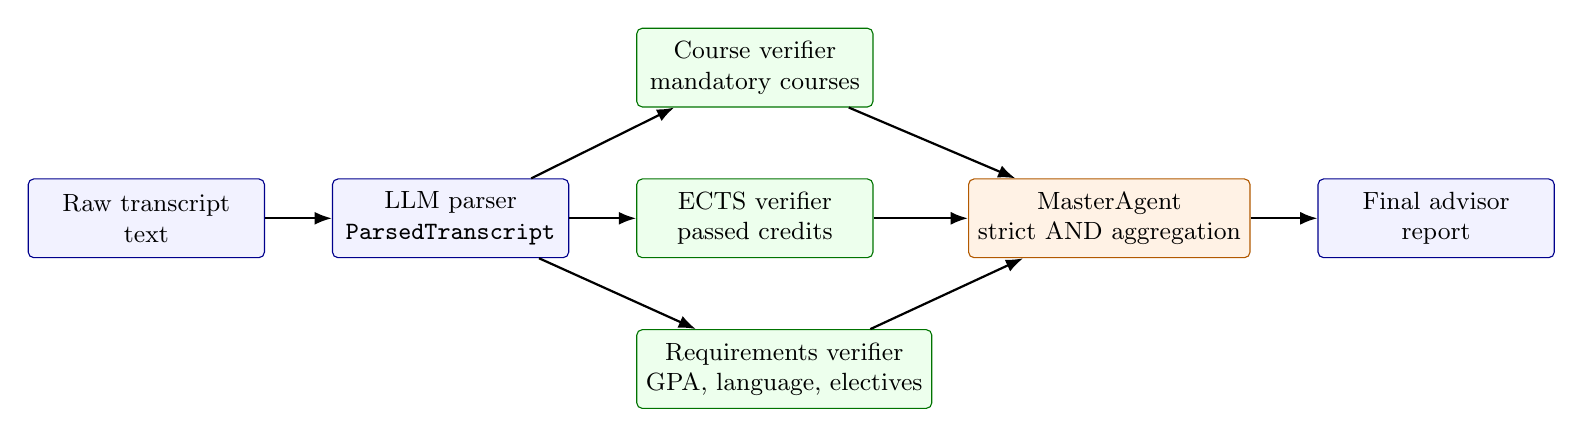
\begin{tikzpicture}[
    node distance=0.9cm and 0.85cm,
    process/.style={
      rectangle,
      rounded corners=2pt,
      draw=blue!55!black,
      fill=blue!5,
      align=center,
      minimum width=3.0cm,
      minimum height=1.0cm,
      font=\small
    },
    verifier/.style={
      rectangle,
      rounded corners=2pt,
      draw=green!45!black,
      fill=green!7,
      align=center,
      minimum width=3.0cm,
      minimum height=1.0cm,
      font=\small
    },
    decision/.style={
      rectangle,
      rounded corners=2pt,
      draw=orange!70!black,
      fill=orange!10,
      align=center,
      minimum width=3.2cm,
      minimum height=1.0cm,
      font=\small
    },
    arrow/.style={-{Latex[length=2.2mm]}, thick}
  ]
    \node[process] (input) {Raw transcript\\text};
    \node[process, right=of input] (parser) {LLM parser\\\texttt{ParsedTranscript}};
    \node[verifier, above right=of parser] (course) {Course verifier\\mandatory courses};
    \node[verifier, right=of parser] (ects) {ECTS verifier\\passed credits};
    \node[verifier, below right=of parser] (requirements) {Requirements verifier\\GPA, language, electives};
    \node[decision, right=1.2cm of ects] (master) {MasterAgent\\strict AND aggregation};
    \node[process, right=of master] (report) {Final advisor\\report};

    \draw[arrow] (input) -- (parser);
    \draw[arrow] (parser) -- (course);
    \draw[arrow] (parser) -- (ects);
    \draw[arrow] (parser) -- (requirements);
    \draw[arrow] (course) -- (master);
    \draw[arrow] (ects) -- (master);
    \draw[arrow] (requirements) -- (master);
    \draw[arrow] (master) -- (report);
  \end{tikzpicture}
  }
  \caption{Hybrid agentic rule-based algorithm used for graduation analysis.}
  \label{fig:algorithmic-approach}
\end{figure}

\section{Decision Logic}

The master decision is intentionally strict. The student is marked eligible for
graduation only if all verifier agents return a passing verdict:

\begin{itemize}
  \item all mandatory courses are satisfied by exact course-code matching or
  official equivalency mappings;
  \item total passed ECTS is at least 240;
  \item GPA is at least 2.00;
  \item language condition is satisfied;
  \item all required elective groups are satisfied;
  \item legacy transition rules do not create unresolved extra obligations.
\end{itemize}

The final output includes both the machine-readable details and the natural
language report. The frontend uses this output to show a high-level decision,
statistics, agent-level evidence, completed mandatory courses, and missing
mandatory courses.

\section{Prompts Used}

The project uses three explicit system prompts in \texttt{backend/agent.py}.
For LaTeX portability, arrows and long dashes are print-normalized below; the
instruction content matches the implemented prompts.

\subsection{Transcript Parser Prompt}

\begin{Prompt}
You are a university transcript parsing expert. Extract ALL courses from a GSU (Galatasaray University) transcript, including failed ones.

The transcript format is tab-separated with semester headers and course rows:

  2021 - 2022 Güz Yarıyılı
  Kodu    Ders Adı    Notu    Kredi    AKTS    Türü
  INF112-B    Programlamaya Giriş    BA    5.0    6    Z
  ...
  AKADEMİK NOT ORTALAMASI    ANO    KREDİ TOPLAMI    AKTS TOPLAMI
  Yarıyıl    2.10    23.5    30.0
  Genel    2.10    23.5    30.0

Column mapping:
- Kodu -> code (course code, may include section suffix like -A, -B, -C -- keep as-is)
- Ders Adı -> name
- Notu -> grade (AA, BA, BB, CB, CC, DC, DD, F, W, DZ, FF, etc.)
- AKTS -> ects (integer)

GPA extraction:
- The cumulative GPA is on the LAST "Genel" row in the transcript, second column (e.g. "Genel    2.49    ..." -> gpa = 2.49)

Skip these rows entirely (do NOT extract as courses):
- "AKADEMİK NOT ORTALAMASI ..." header rows
- "Yarıyıl ..." summary rows
- "Genel ..." summary rows
- Semester header rows (e.g. "2021 - 2022 Güz Yarıyılı")
- Column header rows ("Kodu    Ders Adı ...")

Return ONLY valid JSON matching this exact schema:
{
  "student_name": string or null,
  "student_number": string or null,
  "gpa": number,
  "courses": [
    {"code": string, "name": string, "grade": string, "ects": integer}
  ]
}

Rules:
- Include ALL courses even failed ones (F, FF, DZ, W)
- Course codes must be uppercase
- ects must be an integer (use the AKTS column, not Kredi)
- Return raw JSON only, no markdown, no explanation
\end{Prompt}

\subsection{Master Report Prompt}

\begin{Prompt}
You are the MasterReportAgent for the Computer Engineering department at GSU (Galatasaray University).

Write a concise 2-3 sentence graduation status report in the target language from the user payload.
Base your report strictly on the provided analysis data; do not add or infer anything beyond what is given.

Use advisor-quality academic prose. Do not expose internal machine values, field names, enums, or raw booleans in the report text.
Forbidden report wording includes: true, false, pass, fail, is_graduated, eligible_to_graduate, not_eligible_to_graduate, JSON, boolean.

Interpret the master decision semantically:
- If requirements are satisfied, state that the student meets the graduation requirements.
- If requirements are not satisfied, state that the student does not currently meet the graduation requirements and summarize the main blockers.

Compare courses strictly by course code. Do not infer missing courses from names. A course is only missing if its exact code does not appear in the passed courses list.

Return ONLY valid JSON: {"report": "report text here"}
\end{Prompt}

\subsection{Report Critic Prompt}

\begin{Prompt}
You are the ReportCriticAgent for a university graduation advisor.

Review the draft report against the analysis data and rewrite it if needed.
Preserve the factual decision and all key blockers. Keep it concise, formal, and in the requested target language.

The final report must not contain internal machine values, field names, enums, or raw booleans.
Forbidden report wording includes: true, false, pass, fail, is_graduated, eligible_to_graduate, not_eligible_to_graduate, JSON, boolean.

Return ONLY valid JSON: {"report": "final polished report text here"}
\end{Prompt}

\subsection{Dynamic Tool-Calling Instruction}

During report generation, the master report system prompt is extended with this
instruction:

\begin{Prompt}
You have access to a tool to check the student's history in the database. Use it if a student number is provided. Incorporate any historical progress into your final report JSON.
\end{Prompt}

The available tool is named \texttt{check\_student\_history}. It accepts
\texttt{student\_number} and \texttt{student\_name} parameters and returns a JSON
status such as \texttt{history\_found}, \texttt{no\_history}, or
\texttt{error}. If history is found, the project also creates a frontend-facing
tool log comment comparing previous and current GPA and graduation status.

\section{Testing and Evaluation}

The repository includes both unit-level and scenario-level validation assets:

\begin{itemize}
  \item \texttt{test\_transcript\_validation.py} checks single-transcript
  acceptance and multi-transcript rejection.
  \item \texttt{test\_requirements\_equivalency.py} checks equivalencies,
  failed-grade handling, language requirements, elective groups, and legacy
  transition rules.
  \item \texttt{test\_master\_report\_agent.py} targets report polishing and
  removal of machine-like boolean language.
  \item \texttt{analysis-input-scenarios/} contains 20 named transcript
  scenarios covering positive cases, low GPA, ECTS deficit, missing mandatory
  courses, language failure, modern elective failures, and old-code
  equivalencies.
\end{itemize}

The scenario set is especially valuable because it tests the edge cases that
make academic advising difficult: legacy curricula, old course codes,
replacement rules, and extra elective obligations caused by failed legacy
courses.

\section{Frontend Interface}

The frontend provides the user-facing layer of the Virtual Academic Advisor
system. It is implemented with React and Vite, and it communicates with the
FastAPI backend through the transcript upload, analysis, result retrieval, and
history endpoints. The interface is designed around three main workflows:
submitting a transcript for analysis, inspecting a completed graduation report,
and reviewing previous analyses.

\subsection{Analysis Input Screen}

The analysis screen is the entry point of the application. It allows the user to
paste an unstructured transcript text or upload a plain-text transcript file.
Before sending the transcript to the backend, the frontend performs lightweight
validation to detect empty inputs, unsupported file types, and possible multiple
transcripts in a single submission. This reduces invalid backend calls and gives
the user immediate feedback.

The screen also links the user to the official GSU Computer Engineering
curriculum page, making the academic rule source visible from the interface.
During analysis, the UI displays progress steps such as transcript upload,
parsing, agent evaluation, graduation-condition checking, and report generation.
This makes the agentic pipeline visible to the user instead of presenting the
system as a black-box response generator.

\begin{figure}[H]
  \centering
  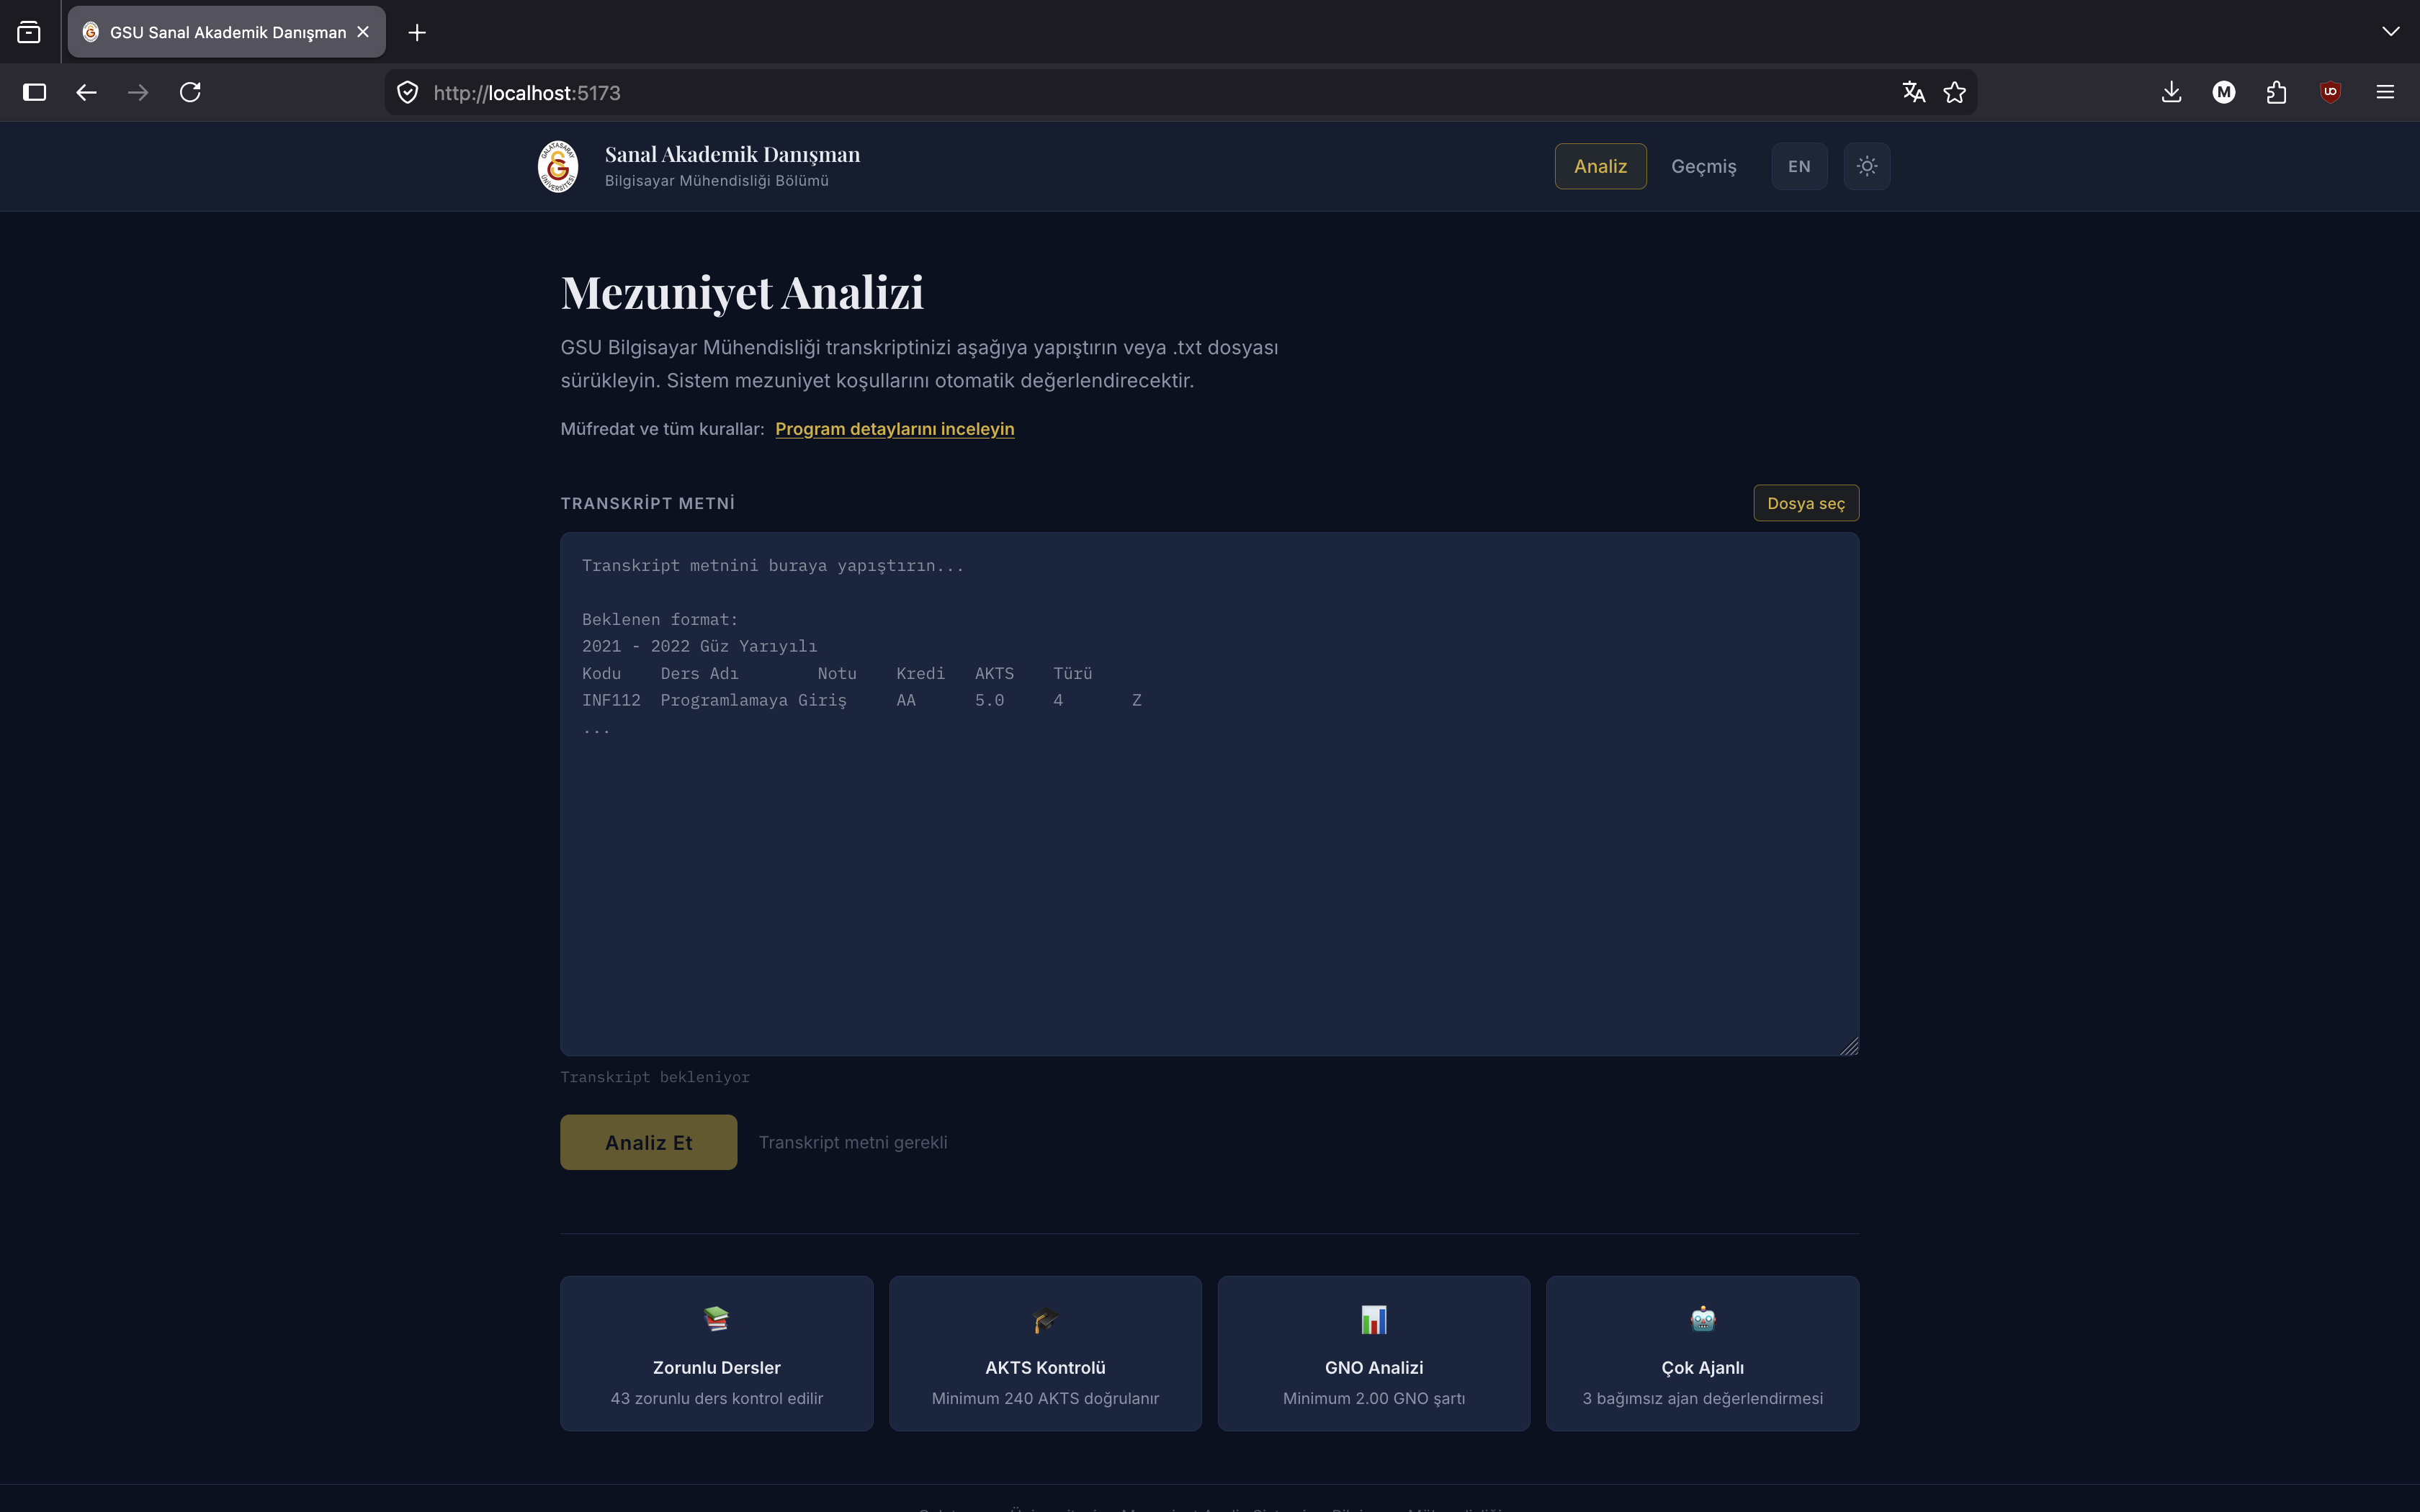
\includegraphics[width=0.90\textwidth]{ui.png}
  \caption{Transcript analysis input screen.}
  \label{fig:ui-analysis}
\end{figure}

\subsection{Analysis Result Screen}

The result screen presents the final graduation decision and the evidence behind
it. At the top of the page, a status banner indicates whether the student is
eligible for graduation or has missing conditions. The LLM-generated advisor
report is displayed directly under this status, while structured metrics such
as GPA, total ECTS, completed mandatory courses, and missing conditions are
shown in separate summary cards.

A key design choice is that the frontend exposes the internal agent verdicts.
The user can inspect the outputs of the CourseVerifierAgent, ECTSVerifierAgent,
RequirementsAgent, and MasterAgent. This supports transparency: the final
decision is not shown as a single unexplained label, but as the result of
multiple specialized agent evaluations. The same page also lists completed and
missing mandatory courses, allowing the student to identify concrete academic
actions needed for graduation.

\begin{figure}[H]
  \centering
  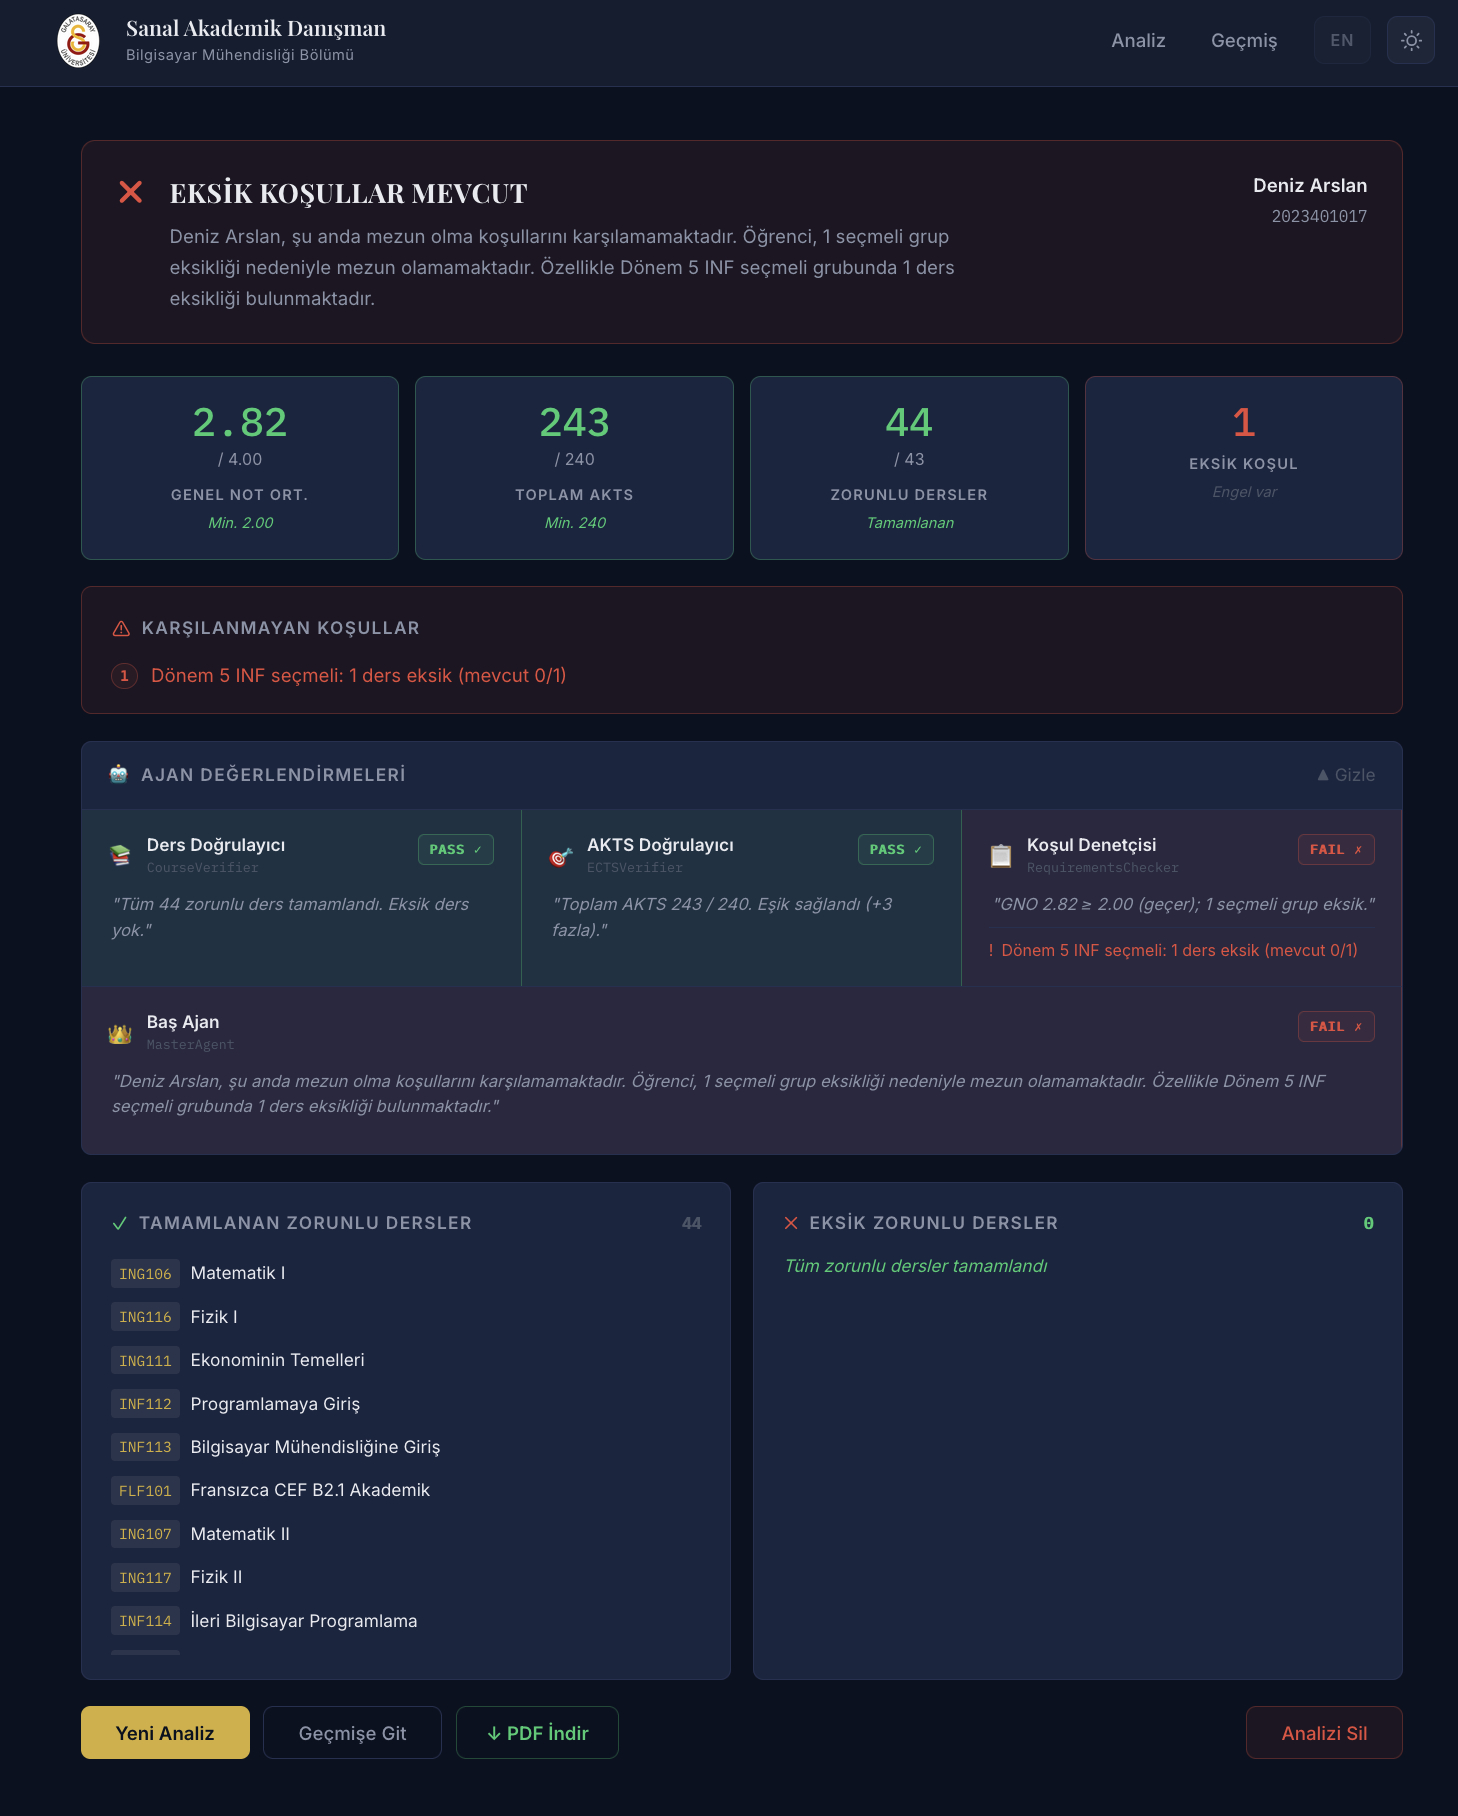
\includegraphics[width=0.90\textwidth]{analyse-result.png}
  \caption{Graduation analysis result screen with agent verdicts and missing conditions.}
  \label{fig:ui-result}
\end{figure}

\subsection{Analysis History Screen}

The history screen provides persistence at the user-interface level. It lists
previously completed analyses with student identity, GPA, ECTS, eligibility
status, and analysis date. The user can search by student name or number, filter
records by graduation status, sort by date, open a previous result, or delete an
analysis.

This screen is also important for the agentic design because the MasterAgent can
query historical records through the \texttt{check\_student\_history} tool
during report generation. Therefore, the frontend history page is not only a
convenience feature; it also reflects the persistent memory layer that can be
used by the tool-augmented reporting agent.

\begin{figure}[H]
  \centering
  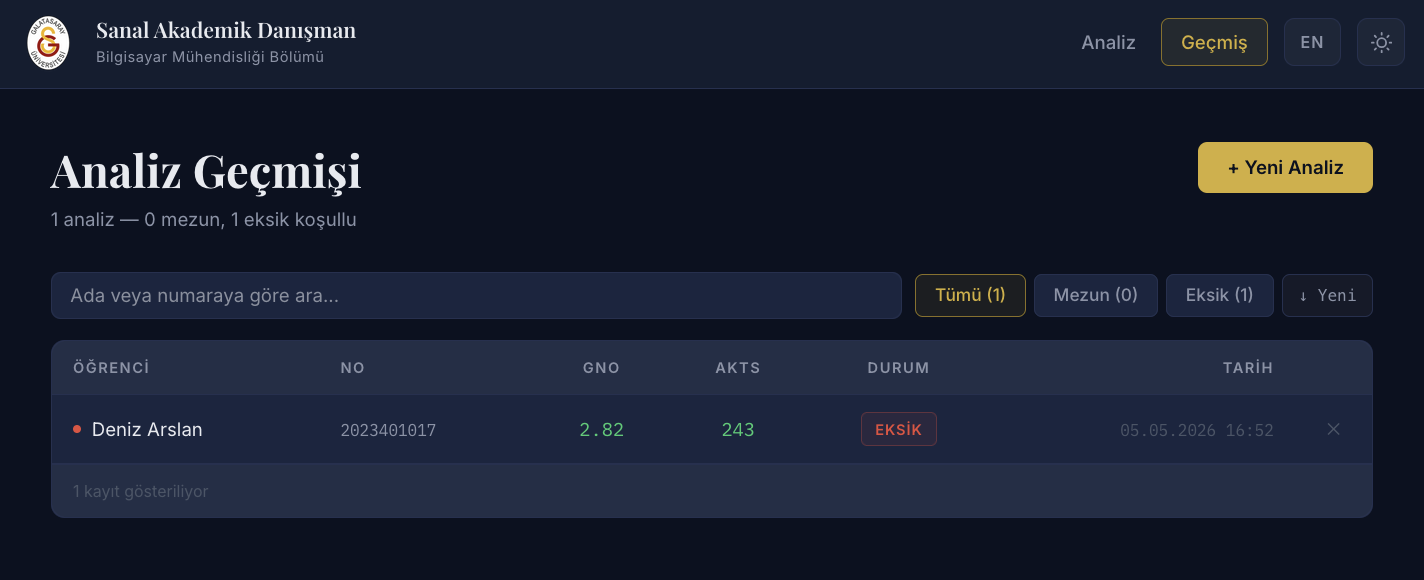
\includegraphics[width=0.90\textwidth]{analyse-history.png}
  \caption{Analysis history screen with search, filtering, and previous results.}
  \label{fig:ui-history}
\end{figure}


\section{Strengths}

\begin{itemize}
  \item The final decision is explainable because each verifier produces a
  verdict, statement, issues list, and details object.
  \item The LLM parser is schema-constrained with Pydantic validation.
  \item GPA extraction has a deterministic override based on the last
  cumulative \texttt{Genel} row.
  \item Course matching is code-based rather than name-based, reducing false
  matches from translated or abbreviated course names.
  \item The system handles section suffixes, failed grades, language
  requirements, elective pools, and old curriculum equivalencies.
  \item Report generation is reviewed by a second LLM role to improve tone and
  remove internal machine terminology.
  \item The UI exposes agent verdicts, making the system more transparent than
  a single opaque eligibility label.
\end{itemize}

\section{Problems Encountered During Development}

Several implementation challenges appeared during the project. The first
challenge was transcript structure. Transcript text contains semester headers,
course rows, summary rows, cumulative GPA rows, and sometimes repeated or
failed courses. Early parsing attempts could confuse summary rows with course
rows or extract GPA from the wrong location. To reduce this risk, the project
uses a strict parser prompt and a deterministic GPA override based on the last
cumulative \texttt{Genel} row.

Another difficulty was course matching. The same course can appear with section
suffixes such as \texttt{-A} or \texttt{-B}, and older students may have course
codes that map to newer curriculum requirements. The verifier logic therefore
normalizes course codes and applies explicit equivalency mappings instead of
matching only by course name. This was important because translated or slightly
different course names can create false matches.

The legacy curriculum rules also made the decision logic more complex than a
simple checklist. Some failed old courses create extra INF or social elective
obligations, and failed grades must not contribute to completed ECTS. These
cases required separate test scenarios and verifier details so that the final
report could explain not only that a student is blocked, but also why.

Finally, some integration issues appeared between the backend and frontend. For
example, the backend requirement list contains 44 mandatory entries while the
frontend result card currently displays a hard-coded denominator of 43. This
does not affect the backend decision, but it showed the importance of keeping
displayed metrics derived from the same source of truth as the verification
logic. The input flow also needed validation against multi-transcript
submissions, because combining more than one transcript in a single request can
produce misleading parsing and analysis results.

\section{Limitations and Future Work}

\begin{itemize}
  \item The curriculum is encoded manually. A future version could scrape or
  import the official ECTS data into a versioned rule database.
  \item The frontend mandatory-course denominator should be aligned with the
  backend requirement count.
  \item The application currently assumes local deployment and does not include
  authentication or role-based access control.
  \item Raw transcript text is stored in SQLite; a production deployment should
  add encryption, retention policy, and stronger privacy controls.
  \item The LLM parser is robust for the expected transcript format, but
  additional OCR/PDF parsing would be needed for scanned transcript uploads.
  \item Prerequisite checking is represented in the official curriculum but is
  not the central graduation-decision criterion in the current implementation.
\end{itemize}

\section{Conclusion}

The project implements a complete Virtual Academic Advisor for GSU Computer
Engineering. Its core contribution is a pragmatic multi-agent architecture:
LLM-backed agents parse and communicate, rule-verifier agents evaluate academic
requirements, and the MasterAgent coordinates evidence, tool use, logging, and
final reporting. This design is well suited to academic advising because it
keeps high-stakes rule decisions traceable while still benefiting from LLM
flexibility for unstructured transcripts and natural-language feedback.

\begin{thebibliography}{9}
\bibitem{gsu-ects}
Galatasaray University ECTS Information System,
\textit{Computer Engineering Undergraduate Program Details}.
\url{https://ects.gsu.edu.tr/tr/program/programmedetails/12}.
Accessed May 9, 2026.

\end{thebibliography}

\end{document}
